\chapter{Implementacija i korisničko sučelje}
		
		
		\section{Korištene tehnologije i alati}
		
			Komunikacija u timu realizirana je korištenjem platforme \underline{Whatsapp}\footnote{\url{https://www.whatsapp.com/}}. 
			Za izradu UML dijagrama korišten je alat \underline{Astah Professional}\footnote{\url{https://astah.net/products/astah-professional/}} i \underline{Visual Paradigm}\footnote{\url{https://online.visual-paradigm.com/}}, a kao sustav za upravljanje izvornim kodom \underline{Git}\footnote{\url{https://git-scm.com/}}. 
			Udaljeni repozitorij projekta je dostupan na web platformi \underline{GitLab}\footnote{\url{https://gitlab.com/}}.
			\par
			Kao razvojno okruženje korišten je \underline{IntelliJ IDEA}\footnote{\url{https://www.jetbrains.com/idea/}} - integrirano razvojno okruženje (IDE) tvrtke JetBrains i \underline{Eclipse}\footnote{\url{https://www.eclipse.org/ide/}}. 
            \par
            Aplikacija je napisana u \underline{Javi}\footnote{\url{https://www.java.com/en/}} koristeći ekosustav \underline{Java Spring}\footnote{\url{https://spring.io/}} za
            izradu backenda te \underline{React}\footnote{\url{https://reactjs.org/}} i jezik \underline{JavaScript}\footnote{\url{https://www.javascript.com/}} za izradu frontenda. 
            \par
            Baza podataka koju smo koristili je (\underline{PostgreSQL}\footnote{\url{https://www.postgresql.org/}}) i ona se nalazi na \underline{pgAdmin}\footnote{\url{https://www.pgadmin.org/}}.

            
            \vspace*{\fill}

			
			
			\eject 
		
	
		\section{Ispitivanje programskog rješenja}
			
Nakon što smo završili s izradom testirali smo rad aplikacije koristeći JUnit tehnologiju i Selenium WebDriver. Testovi su dali zadovoljavajuće rezultate te možemo zaključiti da smo uspjeli implementirati zadane funkcionalnosti.
			
			\subsection{Ispitivanje komponenti}
			
Za ispitivanje komponenti koristili smo JUnit tehnologiju. JUnit okvir je za testiranje komponenti sustava programiranog u Javi. Ispitali smo funkcionalnosti ažuriranja osobnih podataka donora, promjenu optimalnih granica krvi i evidencije krvi slanjem u instituciju. Koriste se objekti tipa UserContoller, BloodController i ConsumptionController na kojima se pozivaju ispitivane funkcionalnosti te UserService, BloodService i RoleService koji su potrebni za dohvaćanje podataka korištenih u funkcijama.
\\\\
\textbf{Ažuriranje osobnih podataka donora}
\\\\
Pozivom funkcije getEditUserInfo iz klase UserController želimo donoru uspješno promijeniti prezime. Na kraju uspoređujemo je li prezime ažuriranog donora jednako željenom novom prezimenu.

\begin{figure}[H]
	\centering
	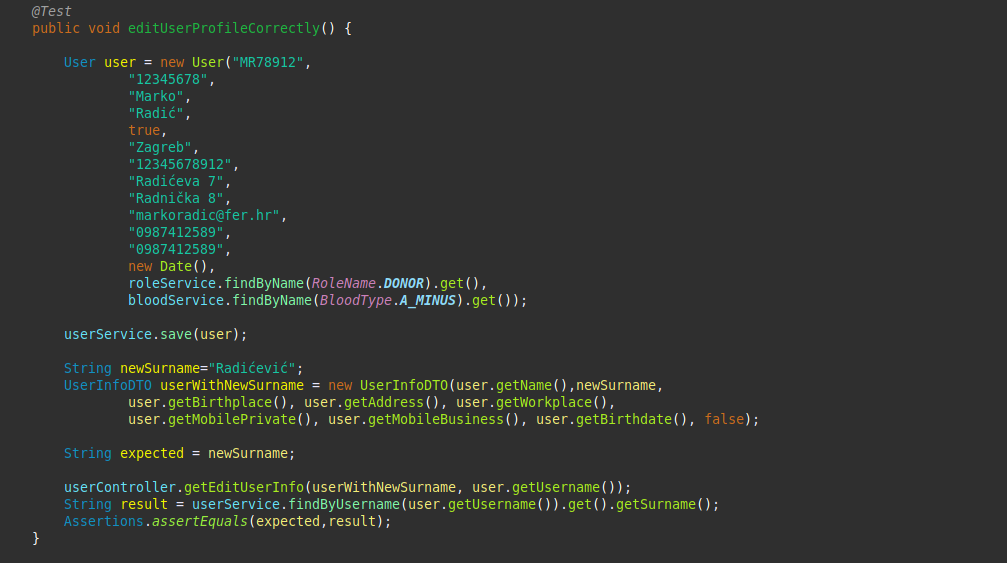
\includegraphics[width=\textwidth, scale=0.5]{slike/unit1}
	\caption{Unit test1}
\end{figure}
{U idućem testu pozivom iste funkcije želimo neuspješno ažurirati polje rejected, koje se ne bi smjelo mijenjati. Na kraju uspoređujemo je li dobivena statusna poruka jednaka očekivanoj "400 BADREQUEST" što bi značilo da aplikacija na pobuđenu situaciju prikladno odgovara.}
\begin{figure}[H]
	\centering
	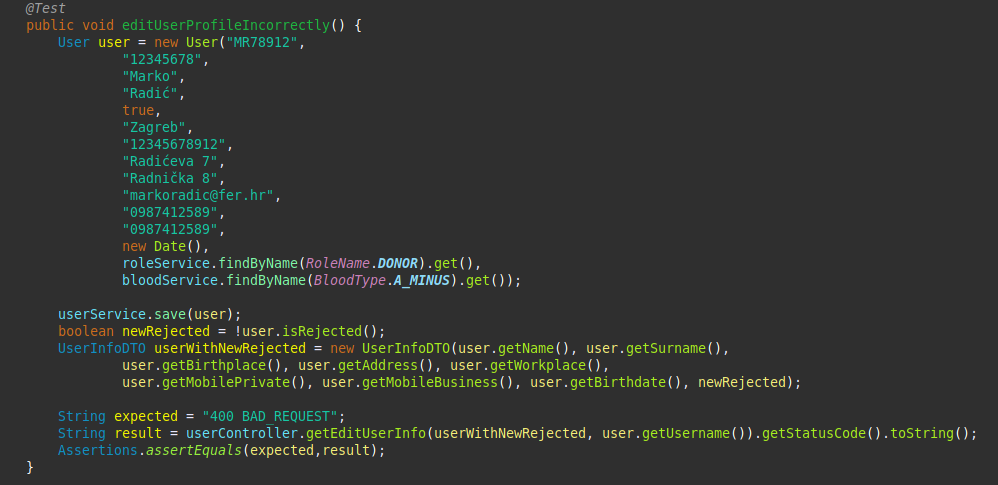
\includegraphics[width=\textwidth, scale=0.5]{slike/unit2}
	\caption{Unit test2}
\end{figure}
\textbf{Promjena optimalnih granica krvi}
\\\\
Pozivom funkcije changeBounds iz klase BloodController želimo uspješno promijeniti donju optimalnu granicu određene krvne grupe. Na kraju uspoređujemo je li donja optimalna granica ažurirane krvne grupe jednaka željenoj granici.
\begin{figure}[H]
	\centering
	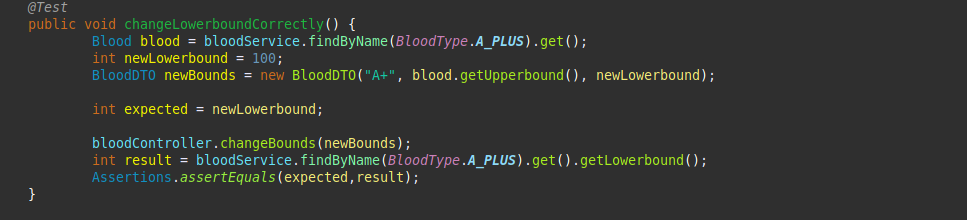
\includegraphics[width=\textwidth, scale=0.5]{slike/unit3}
	\caption{Unit test3}
\end{figure}
\eject
{U idućem testu pozivom iste funkcije želimo neuspješno ažurirati donju optimalnu granicu, koja bi uvijek morala biti pozitivna. Na kraju uspoređujemo je li dobivena statusna poruka jednaka očekivanoj "400 BADREQUEST" što bi značilo da aplikacija na pobuđenu situaciju prikladno odgovara.}
\begin{figure}[H]
	\centering
	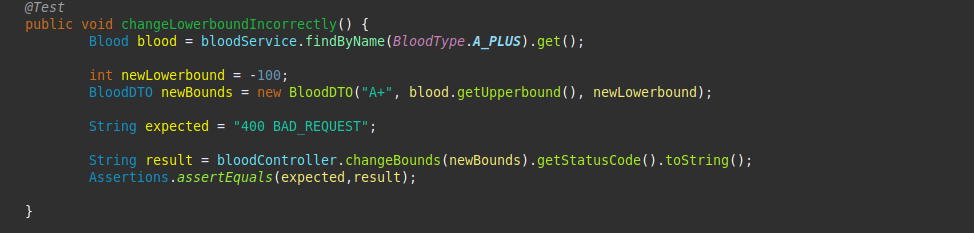
\includegraphics[width=\textwidth, scale=0.5]{slike/unit4}
	\caption{Unit test4}
\end{figure}
\textbf{Evidencija krvi slanjem u instituciju}
\\\\
Pozivom funkcije consumeBlood iz klase ConsumptionController želimo uspješno evidentirati slanje određene krvne grupe u neku instituciju. Na kraju uspoređujemo je li trenutna količina ažurirane krvne grupe jednaka količini umanjenjoj za količinu koja je poslana u instituciju.
\begin{figure}[H]
	\centering
	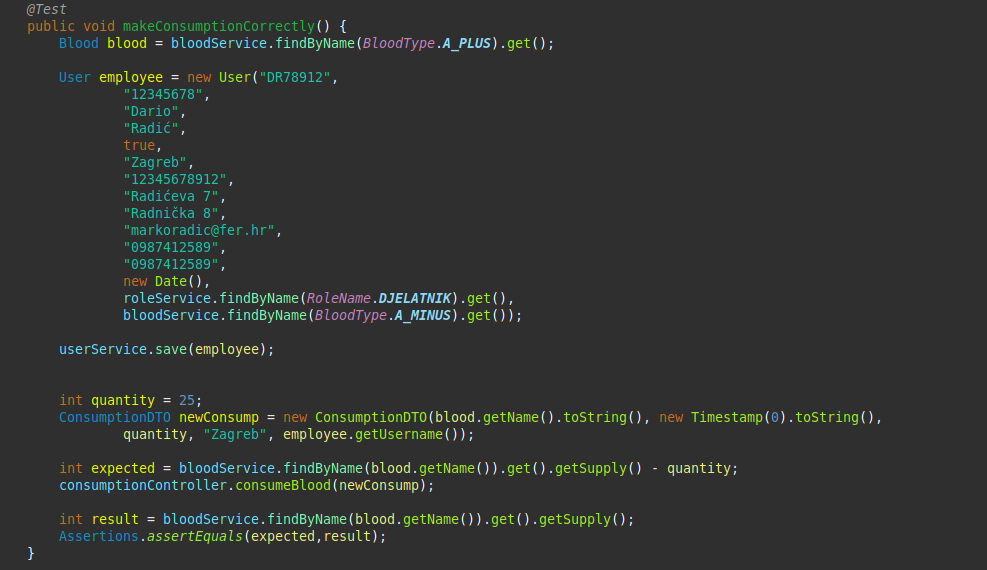
\includegraphics[width=\textwidth, scale=0.5]{slike/unit5}
	\caption{Unit test5}
\end{figure}
\eject	
{U idućem testu pozivom iste funkcije želimo neuspješno evidentirati slanje krvi, čija bi količina uvijek morala biti pozitivna i veća od 0. Na kraju uspoređujemo je li dobivena statusna poruka jednaka očekivanoj "400 BADREQUEST" što bi značilo da aplikacija na pobuđenu situaciju prikladno odgovara. }
\begin{figure}[H]
	\centering
	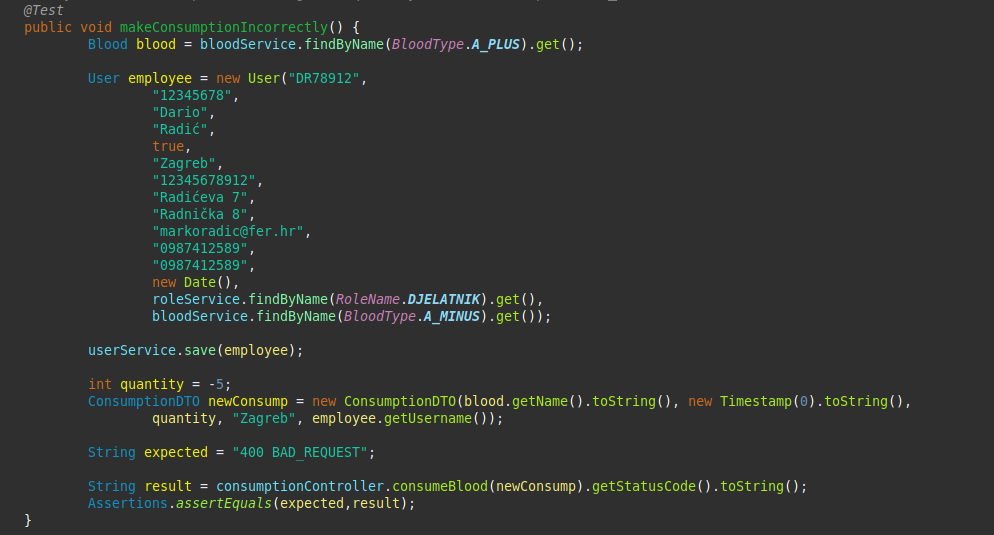
\includegraphics[width=\textwidth, scale=0.5]{slike/unit6}
	\caption{Unit test6}
\end{figure}

\begin{figure}[H]
	\centering
	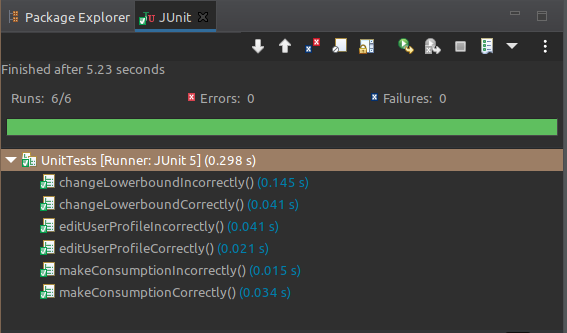
\includegraphics[width=\textwidth, scale=0.5]{slike/unit_testing}
	\caption{Rezultati ispitivanja komponenti}
\end{figure}
\eject
			
			\subsection{Ispitivanje sustava}
			Selenium WebDriver, okvir koji omogućuje programsku interakciju sa internetskim preglednicima, je bio korišten za ispitivanje sustava. Testovi su provedeni na Google Chrome pregledniku. Za sljedeće funkcionalnosti je napravljeno programsko ispitivanje:
			
			 \begin{itemize}
			 	\item {prijava (za donore, djelatnike i admin-a)}
			 	\item {promjene optimalnih granica krvnih grupa (funkcionalnost admin-a)}
			 	\item {evidencija potrošnje krvi (funkcionalnost djelatnika)}
			 	\item {upisivanje donacije u registar (funkcionalnost djelatnika)}
			 	
			 \end{itemize}
		 Korištena je dodatna funkcija za usporavanje sustava, kako se ne bi određeni dijelovi programskog koda za testiranje prerano izvršili:	
\begin{figure}[H]
	\centering
	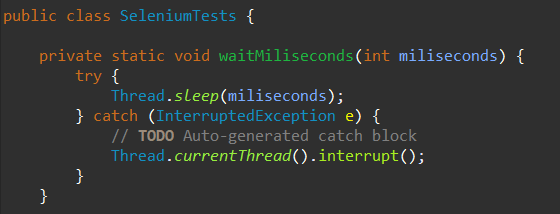
\includegraphics[width=\textwidth, scale=0.5]{slike/wait}
	\caption{Funkcija za usporavanje sustava}
\end{figure}
\eject
\textbf{Prijava}	
\\\\
Ovaj test ima za zadaću ispitati može li se svaka vrsta korisnika sustava ulogirati. Program učitava stranicu i pokušava se ulogirati sa zadanim username­-om i password­-om, te provjera je li doista ulogiran profil za zadani role. Uspjehom se smatra kada je zadani role upisan u drugo polje s desna u gornjoj traci.
\begin{figure}[H]
	\centering
	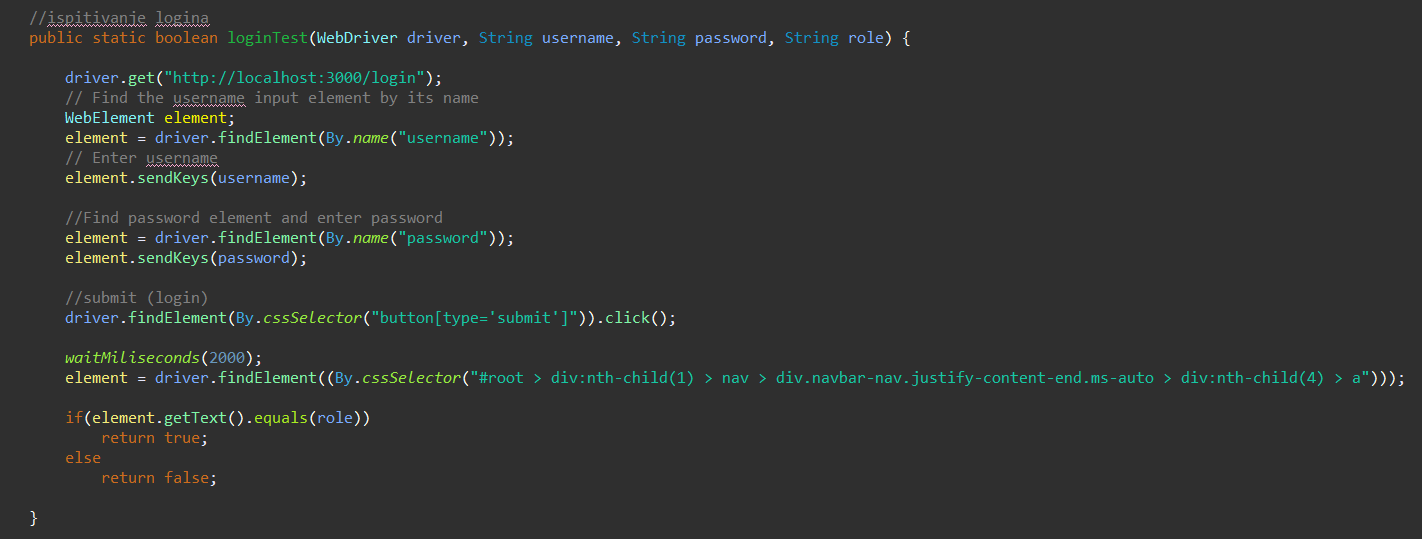
\includegraphics[width=\textwidth, scale=0.5]{slike/selenium1}
	\caption{Selenium test1}
\end{figure}

\textbf{Promjena optimalnih granica krvnih grupa}	
\\\\
Ovaj test ima za zadaću ispitati može li admin postaviti gornju i donju granicu količine krvi određene grupe, koje ako budu pređene dolazi do već spominjanih akcija. Test proglašavamo uspješnim ako poslije pritiska gumba brojevi prikazani u poljima "Gornja" i "Donja" odgovaraju željenima, ako su željene granice pozitivne vrijednosti. Ako pak nisu, onda je test uspješan kada se ispod gumba "Promjeni granice" prikaže poruka "Granice moraju biti pozitivne!".
\eject
\begin{figure}[H]
	\centering
	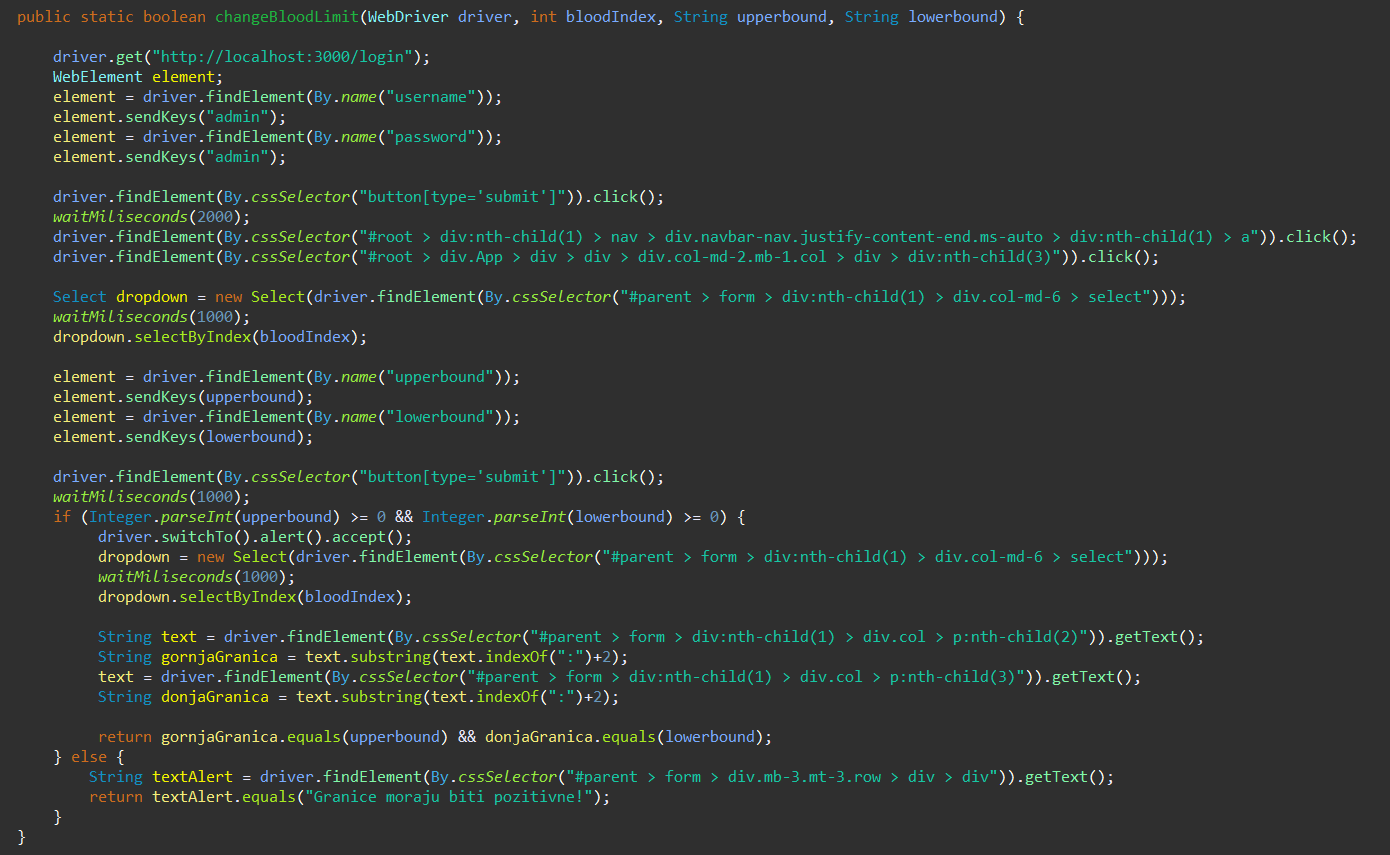
\includegraphics[width=\textwidth, scale=0.5]{slike/selenium2}
	\caption{Selenium test2}
\end{figure}

\textbf{Evidencija potrošnje krvi}	
\\\\
U ovom se testu ispituje može li djelatnik evidentirati slanje krvi u određenu instituciju i odgovara li količina određene krvne grupe u banci nakon slanja očekivanoj količini. Test je uspješan ako je količina krvi određene krvne poslije slanja jednaka očekivanoj. Krv se šalje fiktivnoj lokaciji TESTNA LOKACIJA.
\begin{figure}[H]
	\centering
	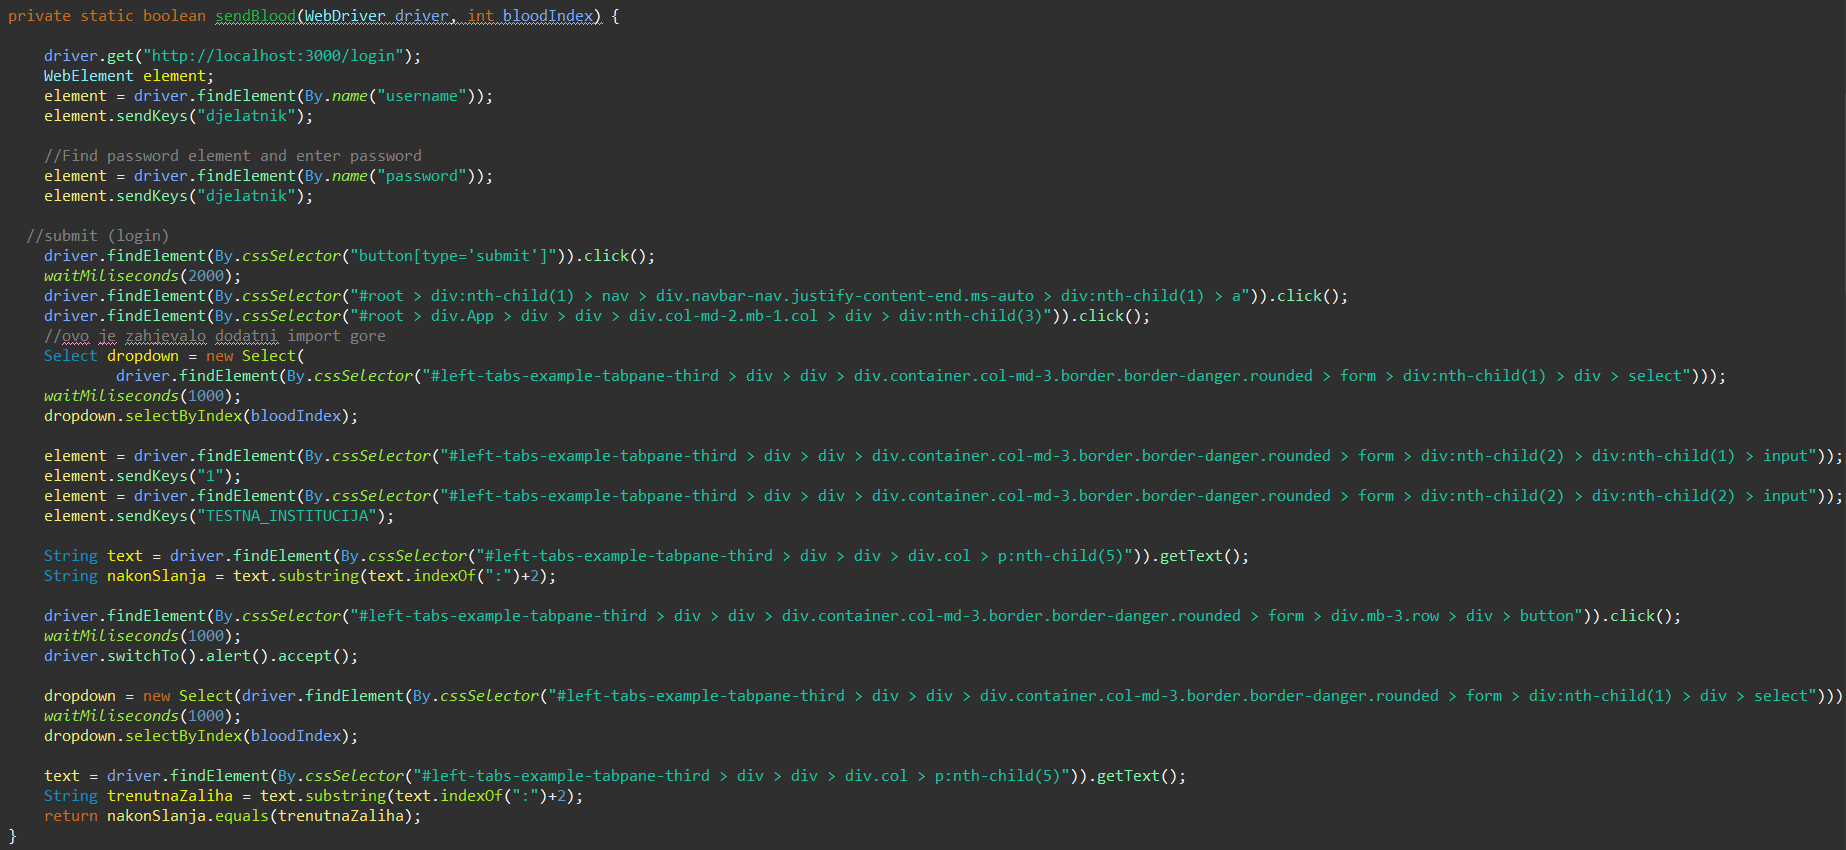
\includegraphics[width=\textwidth, scale=0.5]{slike/selenium3}
	\caption{Selenium test3}
\end{figure}
\eject
\textbf{Upisivanje donacije u registar}	
\\\\
U ovom se testu ispituje može li djelatnik evidentirati obavljenu donaciju (koju je figurativno obavio donor imena TESTDONORNAME na lokaciji TESTLOKACIJA).
Test je prolazan ako preglednik izbaci poruku "Donacija evidentirana" ili "Nije moguće donirati! Nije prošlo dovoljno vremena od zadnje donacije!".
\begin{figure}[H]
	\centering
	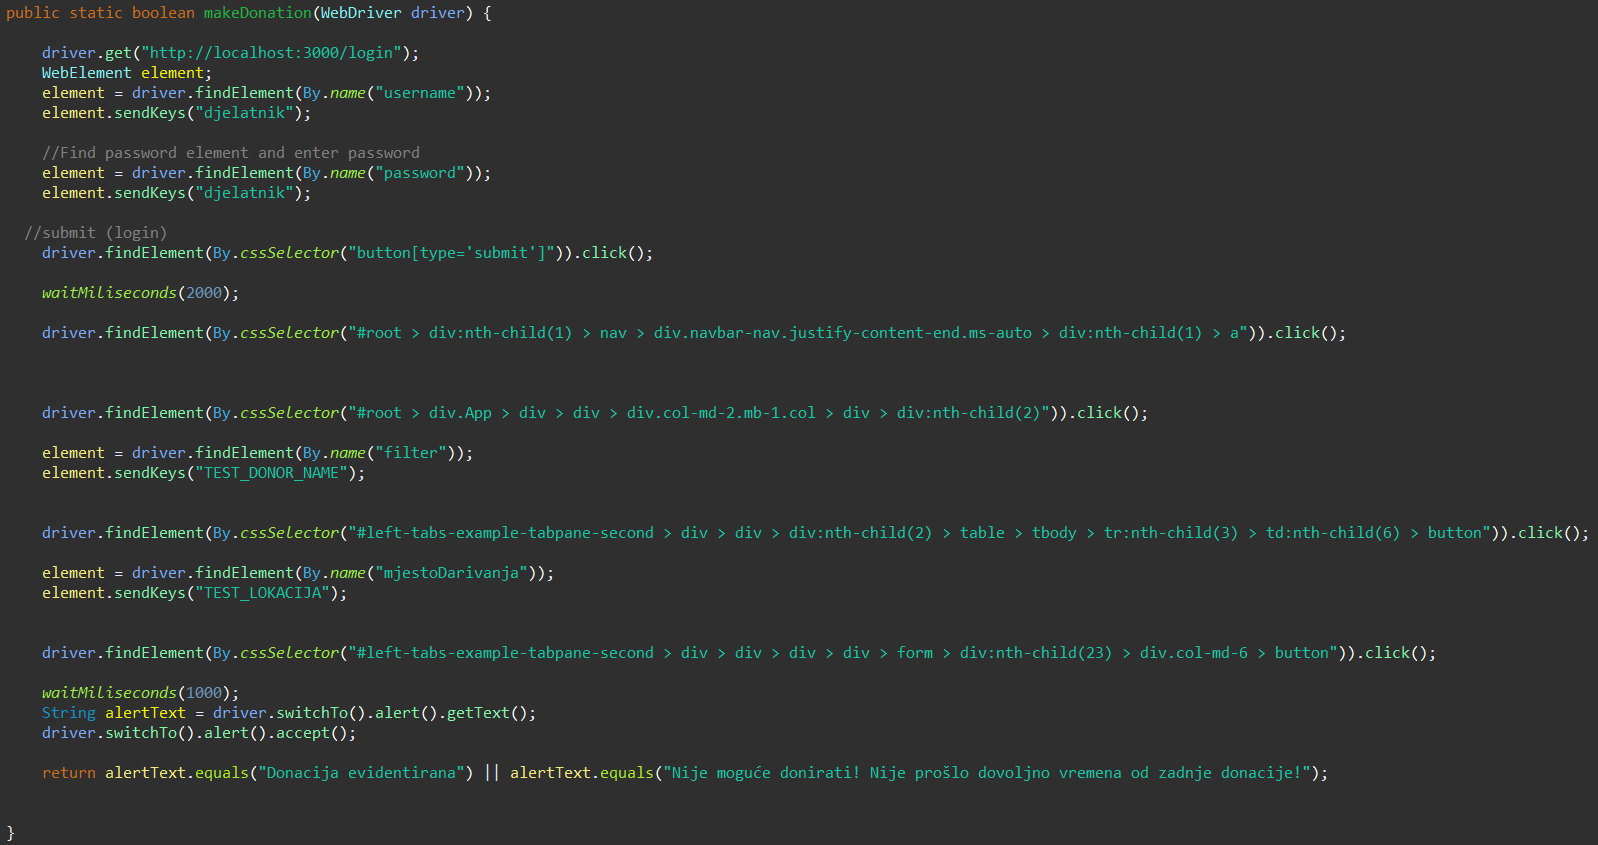
\includegraphics[width=\textwidth, scale=0.5]{slike/selenium4}
	\caption{Selenium test4}
\end{figure}
\eject
Te sve testne funkcije iskoristimo za provođenje testova u glavnoj (main) funkciji:
\begin{figure}[H]
	\centering
	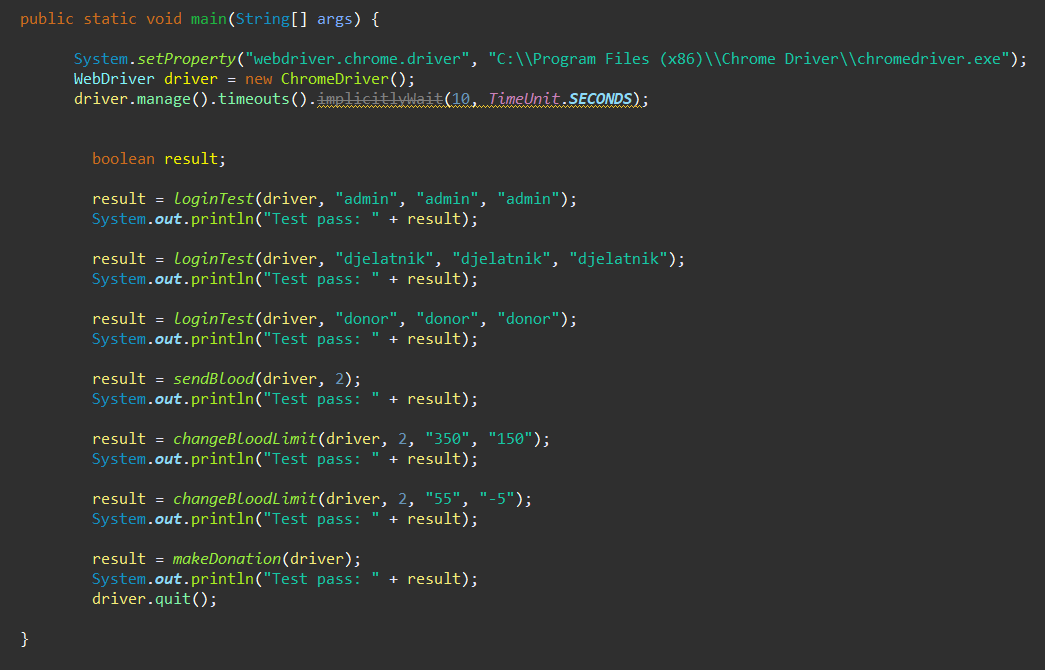
\includegraphics[width=\textwidth, scale=0.5]{slike/main}
	\caption{Funkcija main}
\end{figure}
\begin{figure}[H]
	\centering
	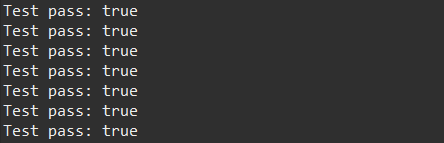
\includegraphics[width=\textwidth, scale=0.5]{slike/rezultat}
	\caption{Rezultat ispitivanja sustava}
\end{figure}
\eject
		\section{Dijagram razmještaja}
			
			Dijagrami razmještaja prikazuju topologiju sustava i odnos sklopovskih i program-
skih dijelova. Olakšavaju nam vizualizaciju razmještaja fizičkog dijela sustava i
sklopovlja. Sustav se sastoji od klijentskog i poslužiteljskog računala. Klijent na
svojem računalu preko web preglednika pristupa aplikaciji. Klijentsko računalo
komunicira s poslužiteljskim računalom preko HTTP veze. Na poslužiteljskom se
računalu nalaze web poslužitelj i poslužitelj baze podataka (PostgreSQL).

\begin{figure}[H]
	\centering
	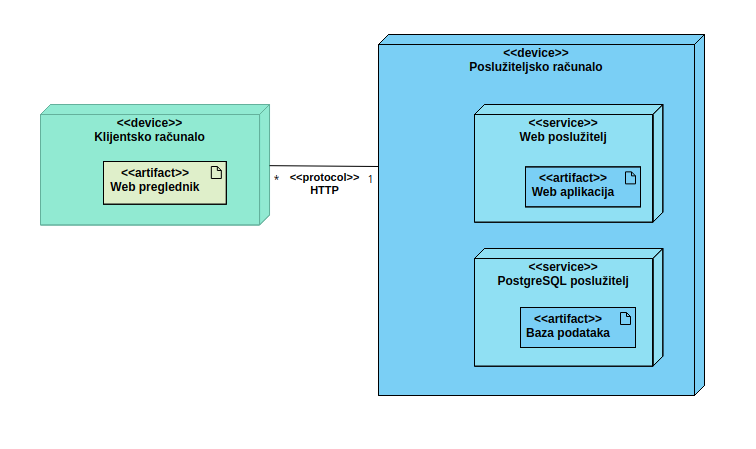
\includegraphics[width=\textwidth, scale=0.5]{dijagrami/dijagram_razmjestaja}
	\caption{Dijagram razmještaja}
	\label{fig:dijagram_razmještaja}
\end{figure}
\eject
	
			
		
		\section{Upute za puštanje u pogon}
		
		Ove upute vrijede te su rađene za Windows Server 2019 desktop experience operativni sustav. Slična (ili gotovo ista) procedura je i za ostale Windows, pa čak i Linux operativne sustave. Većina razlika je u samoj instalaciji potrebnih programskih paketa i runtime-a te postavljanje putanje, nakon čega je konfiguriranje aplikacije i njezino korištenje gotovo identično.
		
			\subsection{Instalacija poslužitelja baze podataka}
			Potrebno je preuzeti {PostgreSQL bazu podataka za Windows x86-64}\footnote{\url{https://www.enterprisedb.com/downloads/postgres-postgresql-downloads/}}. Preporuča se verzija 13.x. Prilikom instalacije preporuča se ostaviti sve (po defaultu) označene komponente za instalaciju, jer će kasnije biti potrebno inicijalno popuniti bazu pomoću pgAdmin4 alata. Odaberite šifru za korisnika postgres te port na kojem će baza podataka slušati zahtjeve. Prilikom završetka instalacije nije potrebno pokretati stack builder. Nakon instalacije (i prilikom svakog restarta servera), Windows automatski pokreće servis baze podataka, te je ona dostupna na prethodno specificiranom portu.
			
			\subsection{Instalacija Node.js runtime-a}
			Potrebno je preuzeti i instalirati {Node.js runtime}\footnote{\url{https://nodejs.org/en/download/}} koji će pokrenuti frontend dio aplikacije. Preporuča se trenutno dostupna LTS verzija (16.13.2 na dan pisanja). Prilikom instalacije potrebno je ostaviti sve (po defaultu) označene komponente za instalaciju, dok ponuđeni alat Chocolatey nije potrebno instalirati. Installer je automatski postavio PATH varijablu okruženja, te su \textit{npm} i \textit{node} naredbe postale globalno dostupne u cmd-u.
			\eject
			\subsection{Instalacija Jave}
			Potrebno je preuzeti i instalirati {JDK paket}\footnote{\url{https://www.oracle.com/java/technologies/downloads/jdk17-windows/}} koji će pokretati backend dio aplikacije.
			
			\begin{figure}[H]
			\centering
			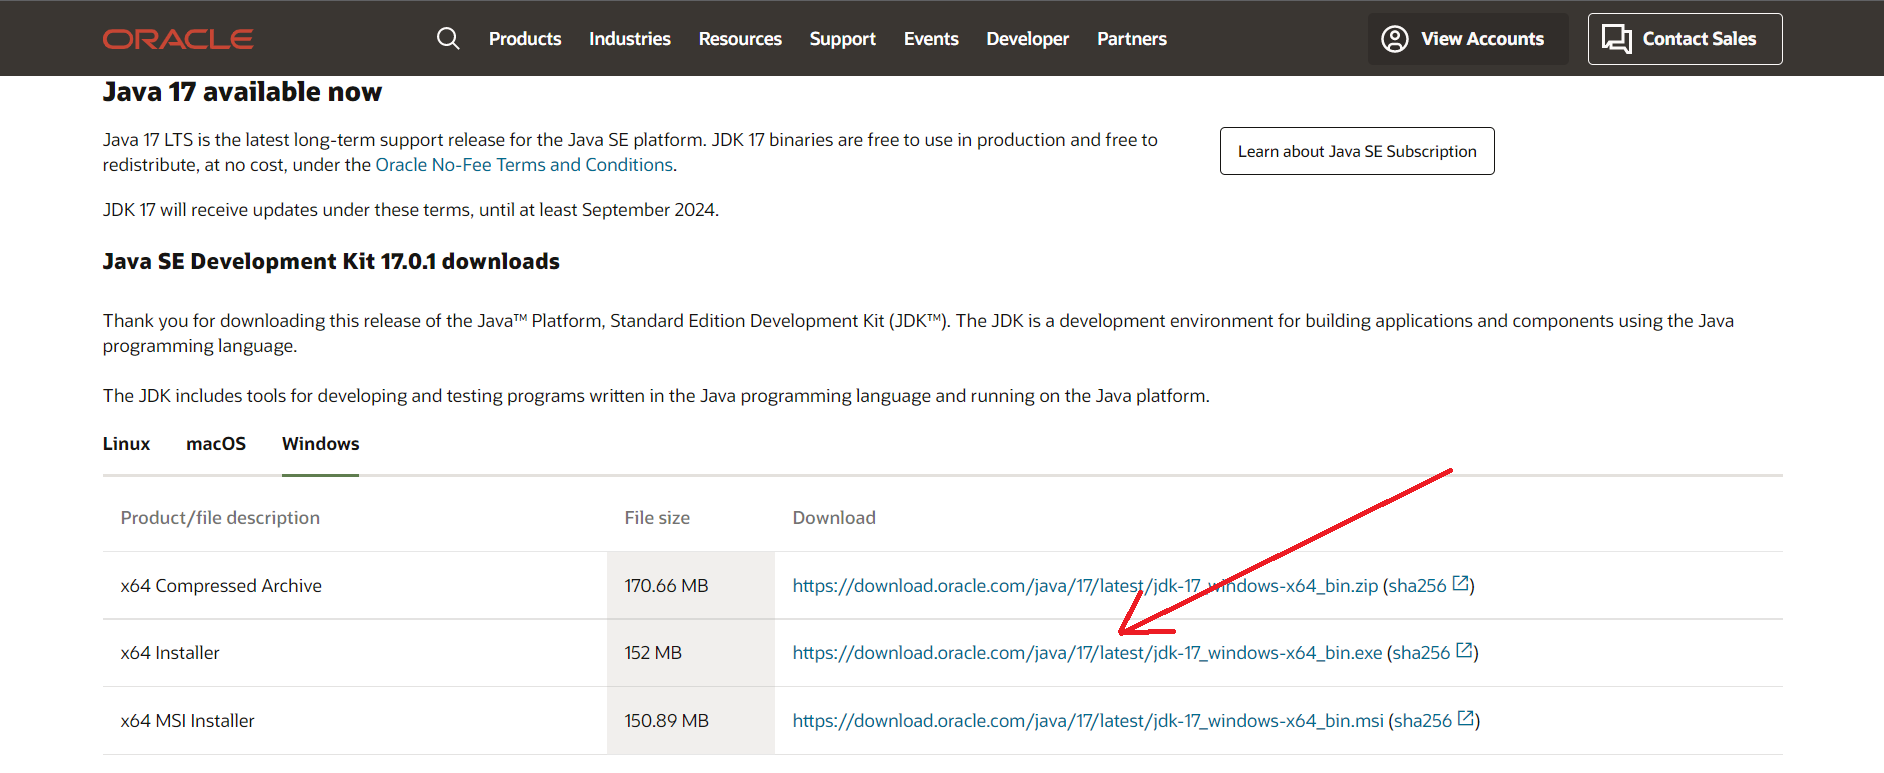
\includegraphics[width=\textwidth, scale=0.5]{slike/JDKdownload}
			\caption{Download JDK17 Installera}
			\label{fig:JDKdownload}
			\end{figure}

			Potrebna je trenutna 17.x.x verzija, no moguće je koristiti i neku od novijih verzija. Installer je automatski postavio PATH varijablu okruženja, te je \textit{java} naredba postala globalno dostupna u cmd-u.
			
			\subsection{Instalacija Maven alata i postavljanje PATH varijable okruženja}
			Potrebno je preuzeti {Maven alat}\footnote{\url{https://maven.apache.org/download.cgi/}} koji služi za kreiranje .jar datoteke iz izvornog koda koja sadrži cijelu backend aplikaciju sa web serverom. Preporuča se 3.8.4 verzija ili novija.
			
			\begin{figure}[H]
			\centering
			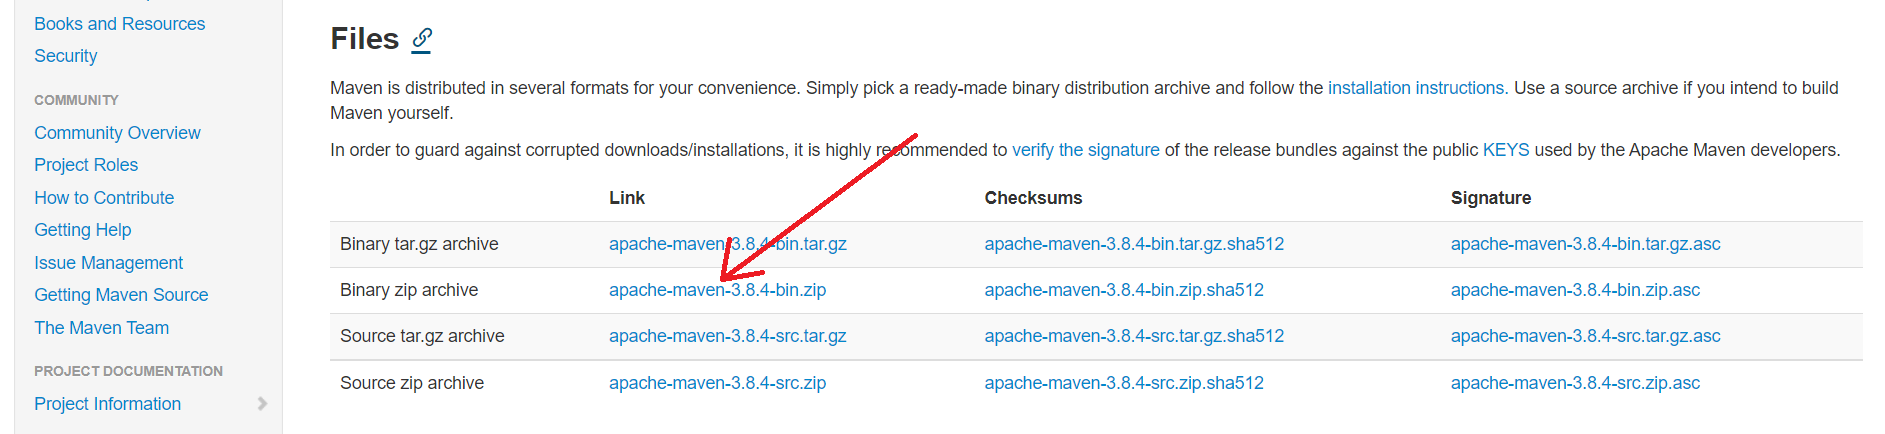
\includegraphics[width=\textwidth, scale=0.5]{slike/mavenDownload}
			\caption{Download Maven Binary-a}
			\label{fig:mavenDownload}
			\end{figure}
			
			\eject
			Nakon preuzimanja potrebno je raspakirati folder u proizvoljnu mapu (u ovom primjeru u \textit{C:/Program Files/apache-maven-3.8.4-bin}) te dodati \textit{bin} folder u PATH varijablu okruženja što se napravi na sljedeći način: 
			Pritiskom \textit{Windows} + \textit{R} tipki otvara se prozor u kojem treba napisati \textit{SystemPropertiesAdvanced} i pritisnuti Enter.
			
			\begin{figure}[H]
			\centering
			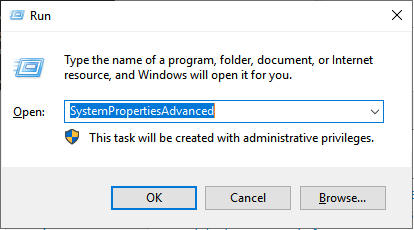
\includegraphics[width=\textwidth, scale=0.5]{slike/RunWindow}
			\caption{Prozor pokreni}
			\label{fig:RunWindow}
			\end{figure}
		
		\eject
			Nakon toga otvara se drugi prozor gdje treba pritisnuti gumb \textit{Environment Variables...}.
			
			\begin{figure}[H]
			\centering
			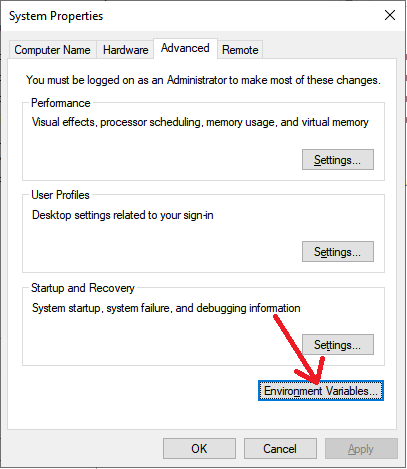
\includegraphics[width=\textwidth, scale=0.5]{slike/SystemPropertiesAdvanced}
			\caption{Prozor naprednih postavka sustava}
			\label{fig:SystemPropertiesAdvanced}
			\end{figure}
			
			\eject
			Time se otvara i treći prozor gdje treba locirati sistemsku \textit{Path} varijablu, označiti ju te pritisnuti gumb \textit{Edit...}
			
			\begin{figure}[H]
			\centering
			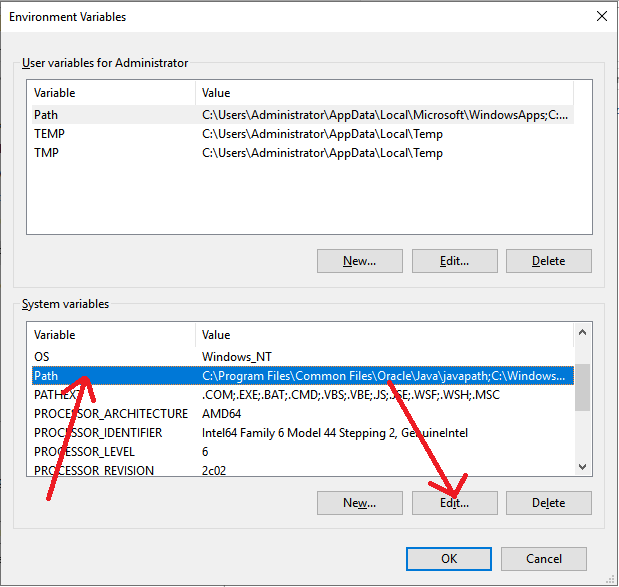
\includegraphics[width=\textwidth, scale=0.5]{slike/EnvironmentVariables}
			\caption{Prozor varijabli okruženja}
			\label{fig:EnvironmentVariables}
			\end{figure}
			
			\eject
			Nakon toga, u novootvorenom prozoru, pritiskom na tipku \textit{New} potrebno je napisati putanju do \textit{bin} foldera prethodno raspakiranog Maven alata. U ovom slučaju to je \textit{C/Program Files/apache-maven-3.8.4-bin/apache-maven-3.8.4/bin}.
			
			\begin{figure}[H]
			\centering
			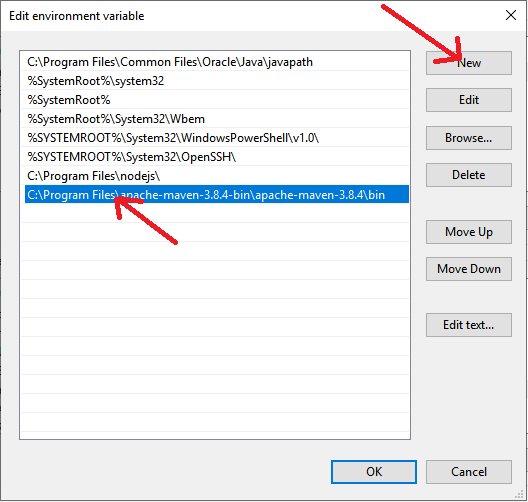
\includegraphics[width=\textwidth, scale=0.5]{slike/newPathInsert}
			\caption{Nova putanja u PATH varijabli okruženja}
			\label{fig:newPathInsert}
			\end{figure}
			
			\eject
			\subsection{Podešavanje i pokretanje backend dio aplikacije te inicijalno punjenje baze}
			Kako bi aplikacija ispravno radila, potrebno je postaviti parametre za povezivanje s bazom podataka te ispravnu IP adresu i port za aktivacijski link u datoteci \textit{application.properties} (koja se nalazi na putanji \textit{IzvorniKod/trueblood/src/main/resources}).
			
			\begin{figure}[H]
			\centering
			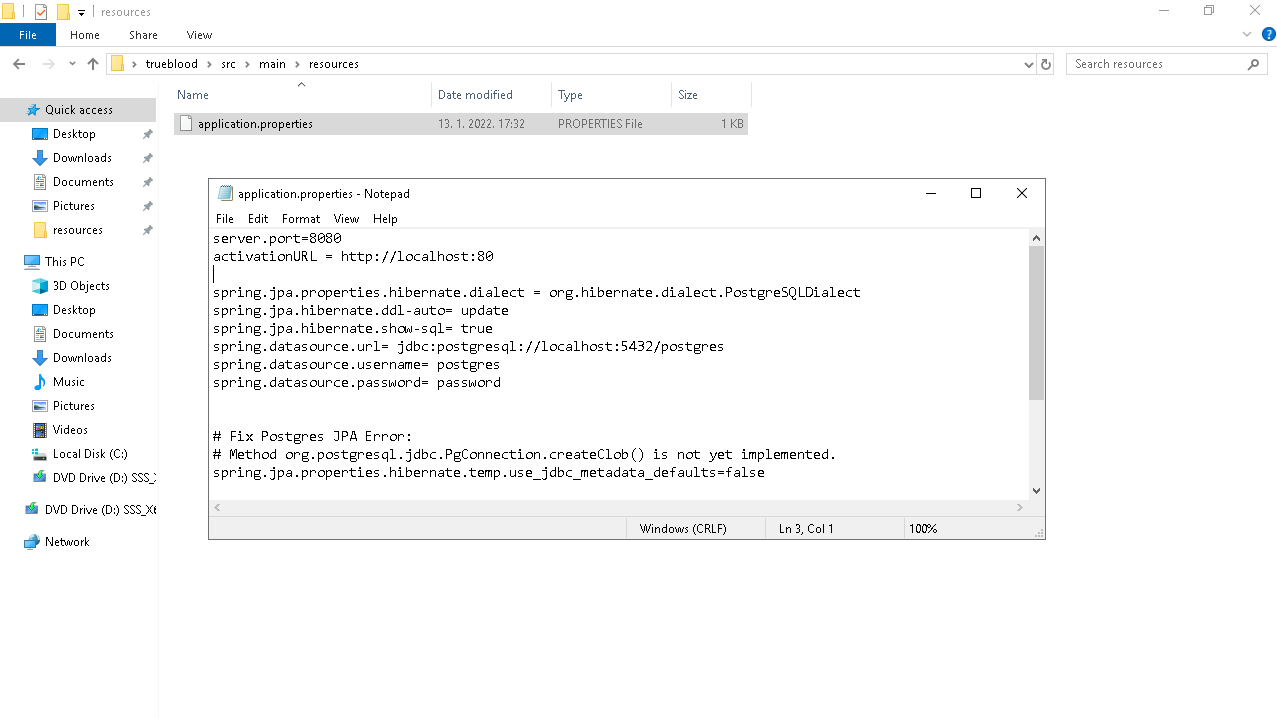
\includegraphics[width=\textwidth, scale=0.5]{slike/ApplicationProperties}
			\caption{application.properties datoteka}
			\label{fig:ApplicationProperties}
			\end{figure}
			
			Na samom vrhu nalazi se konfiguracijska linija \textit{server.port=8080} kojom se može promijeniti port backend servera (default je 8080).
			Ispod toga, nalazi se linija \textit{activationURL = http://localhost:80}. Ovdje je potrebno specificirati javnu IP adresu servera (ili DNS name tj. link ukoliko se koristi), te port frontend dijela aplikacije (ukoliko nije default 80). Jedan od načina kako se to može napraviti jest tako da se na serveru otvori stranica \textit{https://www.whatismyip.com/} te se kopira ispisana IP adresa na mjesto (activationURL = \textit{http://IPadresa:80})
			
			\eject
			
			\begin{figure}[H]
			\centering
			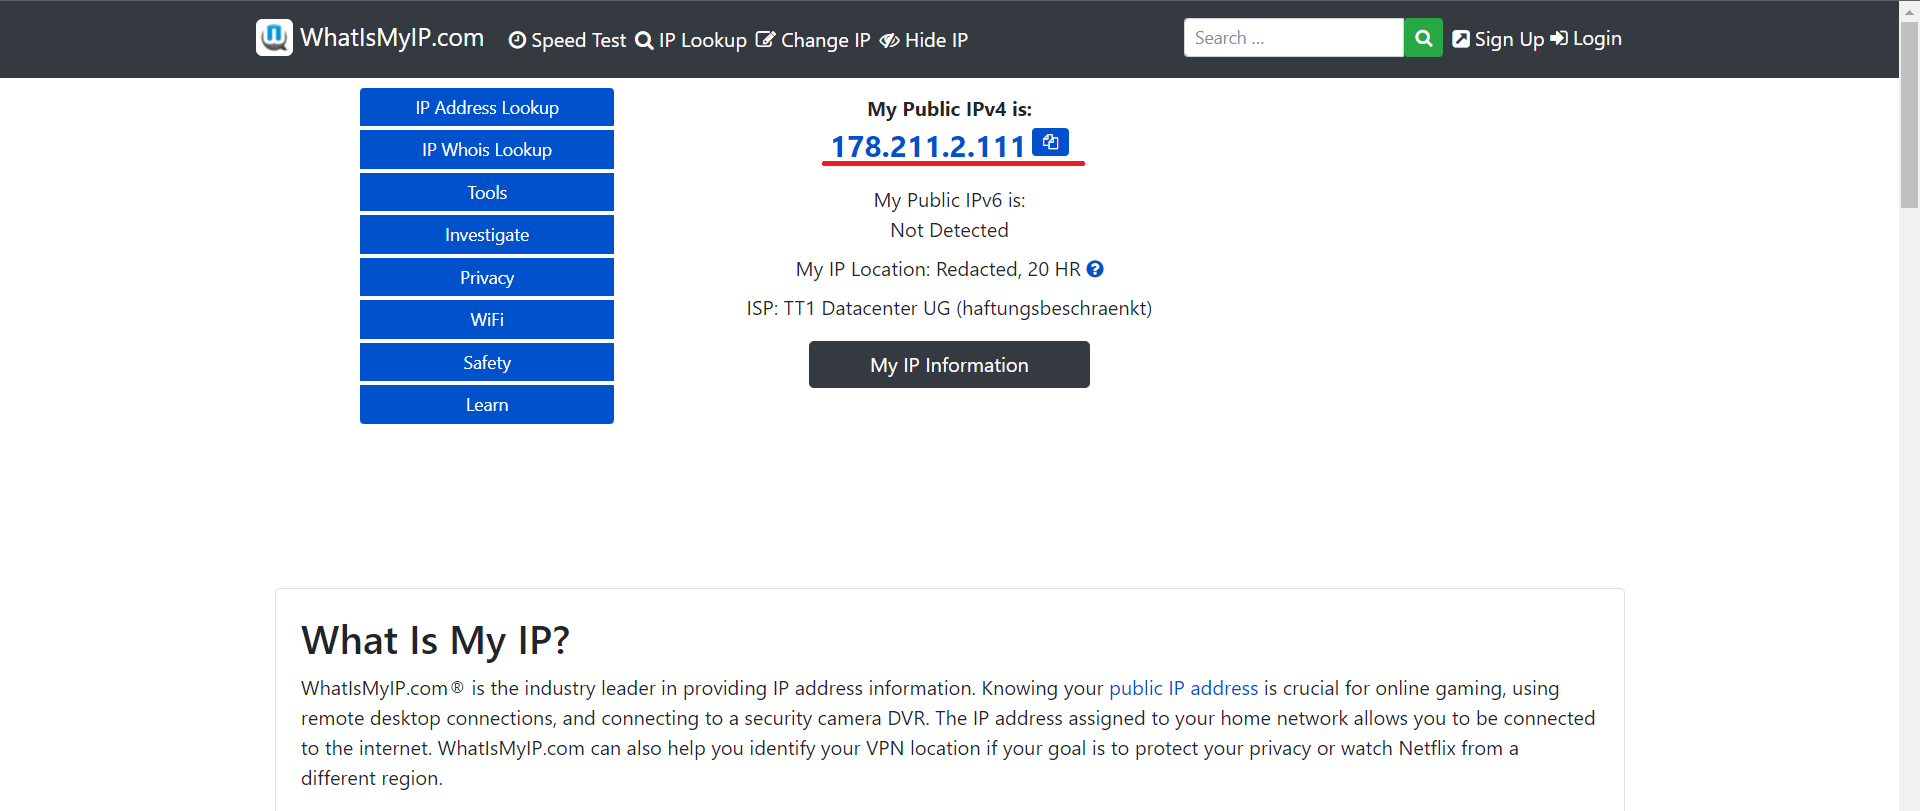
\includegraphics[width=\textwidth, scale=0.5]{slike/WhatIsMyIp}
			\caption{Kopiranje javne IPv4 adrese servera}
			\label{fig:WhatIsMyIp}
			\end{figure}

			Nadalje, ispod se nalaze 3 ključne linije za povezivanje s bazom:
			\begin{itemize}
				\item{\textit{spring.datasource.url= jdbc:postgresql://localhost:5432/postgres}}
				\item{\textit{spring.datasource.username= postgres}}
				\item{\textit{spring.datasource.password= password}}
			\end{itemize}			
			
			Na prvoj liniji je potrebno specificirati odabrani port prilikom instalacije 
			\textit{../localhost:portnumber/...}, te ime baze \textit{...5432/imebaze} ukoliko se ne koristi default baza.
			Na drugoj liniji specificira se ime korisnika kojeg aplikacija koristi za pristup bazi, te na trećoj liniji lozinka tog korisnika. Ukoliko se koristi default \textit{postgres} korisnik za koji je definirana lozinka prilikom instalacije, ovdje se upiše ta ista lozinka.\\
			
			Nakon modificiranja i spremanja konfiguracijske datoteke, potrebno je otvoriti cmd, pozicionirati se u trueBlood folder \textit{IzvorniKod/trueBlood} te izvršiti komandu \textit{mvn clean install -DskipTests} kojom će Maven alat preuzeti potrebne dependency-je te izraditi .jar datoteku spremnu za pokretanje.
			\eject
			
			\begin{figure}[H]
			\centering
			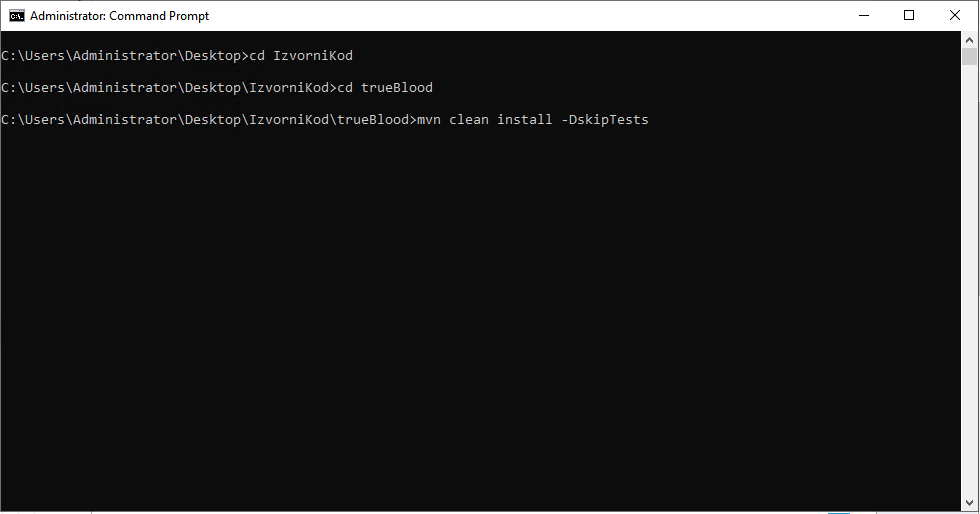
\includegraphics[width=\textwidth]{slike/CmdCommands}
			\caption{Pozicioniranje i izvršavanje komandi}
			\label{fig:CmdCommands}
			\end{figure}
				
			\begin{figure}[H]
			\centering
			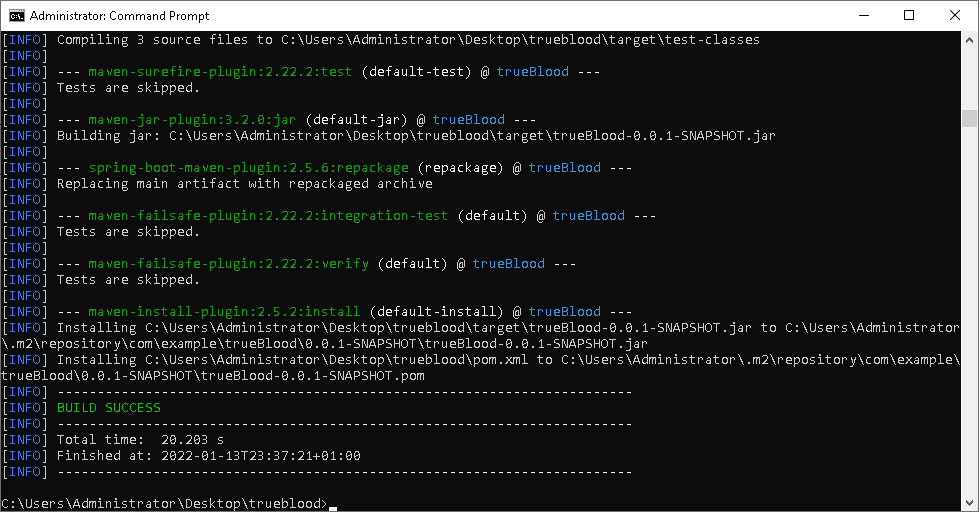
\includegraphics[width=\textwidth]{slike/cmdBuildFinished}
			\caption{Završni izlaz nakon uspješnog builda aplikacije}
			\label{fig:cmdBuildFinished}
			\end{figure}
			\eject
			Izrađena .jar datoteka (koja u sebi sadrži sve što je potrebno za njezino pokretanje, uključujući i Tomcat web server) nalazi se na putanji \textit{IzvorniKod/trueBlood/target} pod imenom \textit{trueBlood-0.0.1-SNAPSHOT}, te se sa cmd-om potrebno pozicionirati u navedeni folder i izvršiti komandu \textit{java -jar trueBlood-0.0.1-SNAPSHOT.jar} čime se pokreće backend dio aplikacije. Potrebno je ostaviti otvoren cmd prozor kako bi aplikacija radila.\\\\
			
			Aplikacija sama stvara tablice i strukturu podataka u schemu \textit{public} unutar baze specificirane u \textit{application.properties}. No za ispravan rad potrebno je još dodavanje statičkih redova na način da se otvori prije instalirana aplikacija PgAdmin, desnim klikom na korištenu bazu odabere se \textit{Query Tool}, te u tekstni prozor se kopira sadržaj datoteke \textit{puniteljBaze.sql} (koja se nalazi na putanji \textit{IzvorniKod/trueblood/puniteljBaze.sql}). Ovim početnim punjenjem baze podataka, definira se početni admin korisnički račun (username: \textit{admin}, password: \textit{admin}) pomoću kojeg je moguće daljnje upravljanje aplikacijom.
			
			\begin{figure}[H]
			\centering
			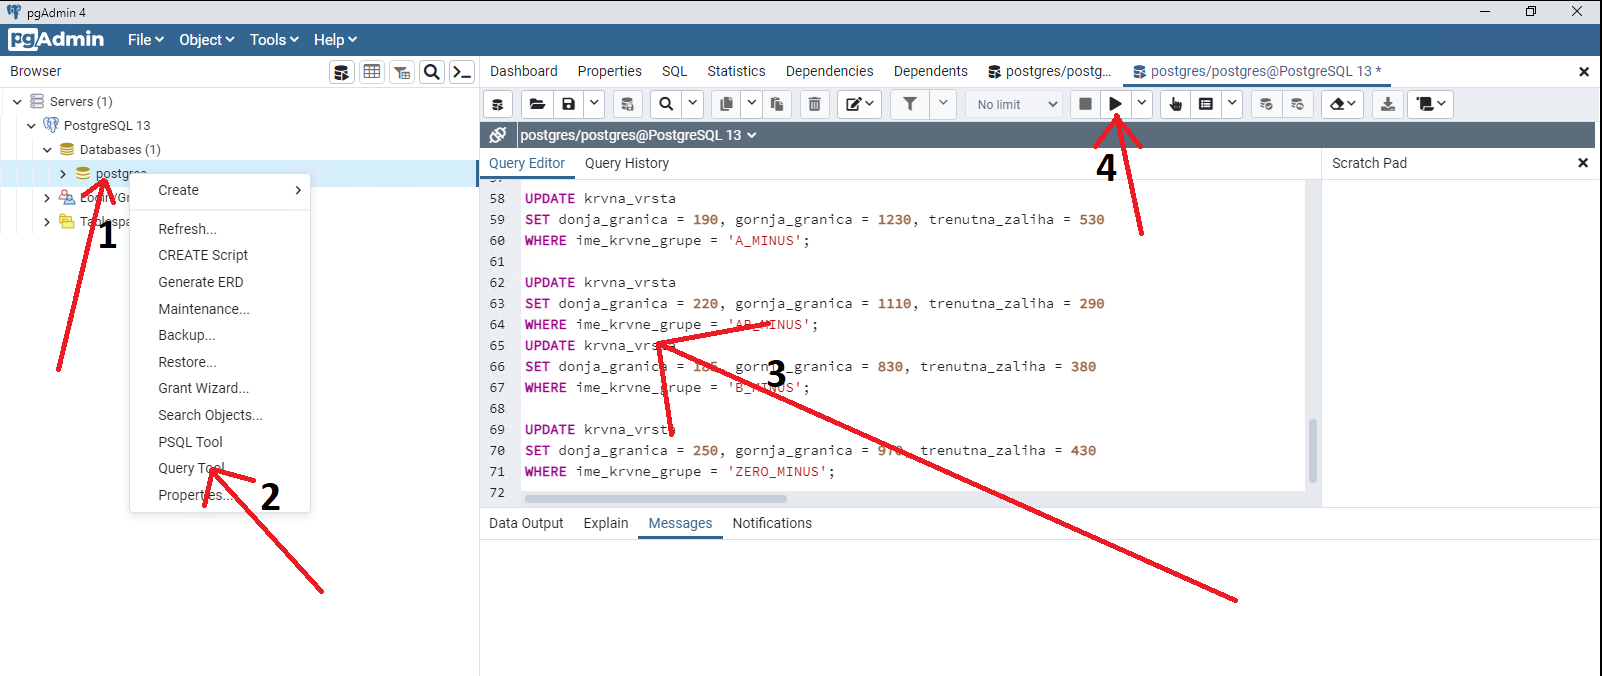
\includegraphics[width=\textwidth, scale=0.5]{slike/puniteljBaze}
			\caption{Punjenje baze statičkim podacima}
			\label{fig:puniteljBaze}
			\end{figure}
			\eject
			\subsection{Podešavanje i pokretanje frontend dijela aplikacije}
			Nakon uspješno pokrenutog backend dijela aplikacije, potrebno je još posložiti i pokrenuti i frontend dio aplikacije. Potrebno je javnu IP adresu servera i port backend dijela aplijacije (definiranog prije u \textit{application.properties}) upisati u datoteku \textit{Constants.js} koja se nalazi na putanji \textit{IzvorniKod/trueBlood/frontend/src/components} na liniji \textit{export const SPRINGURL = 'http://localhost:8080'}.
		
			\begin{figure}[H]
			\centering
			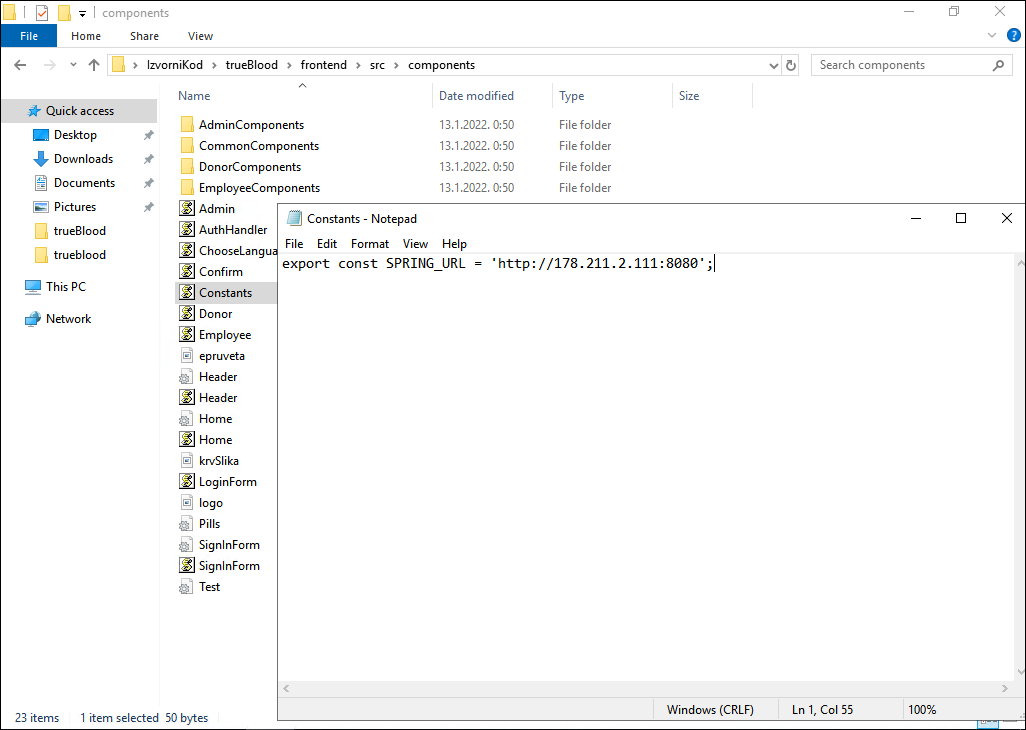
\includegraphics[width=\textwidth, scale=0.5]{slike/ConstantsJs}
			\caption{Constants.js datoteka}
			\label{fig:ConstantsJs}
			\end{figure}
			\eject
			Nakon modificiranja i spremanja datoteke Constants.js, potrebno je otvoriti novi cmd prozor, pozicionirati se u frontend folder (putanja \textit{IzvorniKod/trueBlood/frontend}) te izvršiti komandu \textit{npm install} kojom se instaliraju potrebni node moduli. Zatim komandu \textit{npm run build} kojom se kreira folder u kojem se nalaze izvršne datoteke spremne za korištenje u produkciji. Te datoteke mogu se upogoniti u bilo kojem proizvoljnom web serveru (poput microsoftovog IIS-a), no radi jednostavnosti, nakon izvršenja prethodne naredbe, naredbom \textit{npm install -g serve} dodatno se instalira \textit{serve} modul, koji koristi za posluživanje prije kreiranih datoteka. Napokon, naredbom \textit{serve -s build -l 80} pokreće se Node.js web server na portu 80, te je ovime kompletna aplikacija spremna za upotrebu.
			
			\subsection{Napomene}
			
			Ukoliko je uključen, potrebno je odabrane portove frontend i backend dijela aplikacije propustiti kroz firewall.\\\\
			Ukoliko nakon pokretanja backend ili frontend dijela aplikacije neki od njih izgledno ne radi, moguće da se slučajnim lijevim klika mišom na cmd prozor (koji ga pokreće taj dio aplikacije zamrznuo. Potrebno je na taj isti prozor pritisnuti desni klik miša, što će nastaviti rad zamrznutog dijela aplikacije. Preporuča se minimiziranje cmd prozora kako ne bi došlo do tog problema.
			
			
			\eject